\section{Implémentation}

\subsection{Hiérarchie complète}
\label{sec:sig-hierarchy}

La figure \ref{sec:sig-hierarchy} présente la hiérarchie formée par les différentes classes de signaux. Cette section aborde plus en détails les spécificités de chacune d'elles.

\begin{figure}[h]
	\centering
	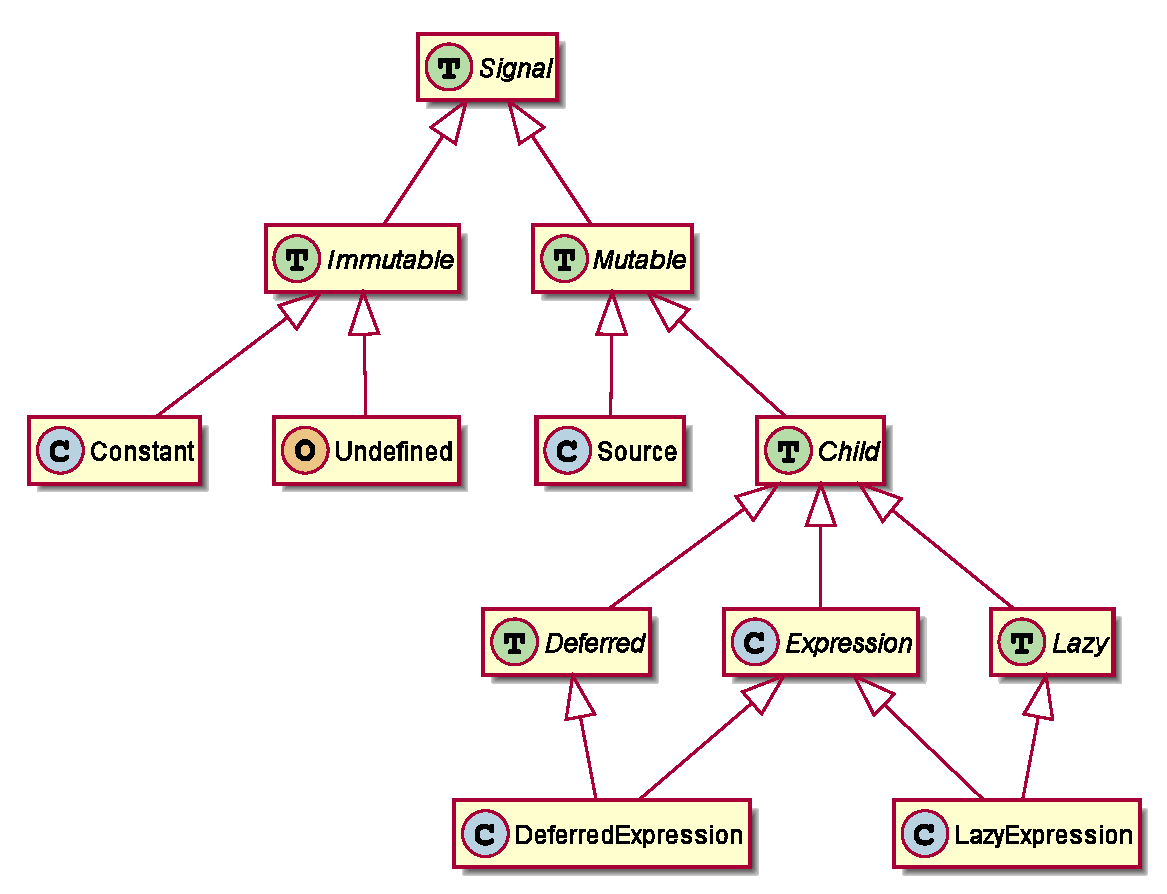
\includegraphics[width=10cm]{img/sig_hierarchy.eps}
	\caption{Hiérarchie des signaux}
	\label{fig:sig-hierarchy}
\end{figure}

\textit{Chaque trait entre Signal et la classe finale d'implémentation précise une sémantique indéfinie sur trait supérieur et ajoute une nouvelle méthode à définir par les types inférieurs:}
\begin{itemize}
	\item \texttt{Signal}: fonction \texttt{def option: T} indéfinie. Doit retourner la valeur courante du signal.
	\item \texttt{Immutable}: redéfini \texttt{option} en \texttt{val} puisque l'état est immutable.
	\item \texttt{Constant}: défini \texttt{val option = Some(value)}
	\item \texttt{Undefined}: défini \texttt{val option = None}
	\item \texttt{Mutable}: déclare la méthode abstraite \texttt{def current: Option[T]}, représentant également l'état du signal mais dont le nom indique clairement la sémantique mutable.
	
	Défini la méthode \texttt{option} en se basant sur \texttt{current} mais y ajoute la détection automatique des signaux enfants. De cette façon toutes les méthodes de \texttt{Signal} en utilisant \texttt{current} obtiennent également les mécanisme de détection.
	
	Défini la méthode \texttt{notifyChildren()} utilisée pour signaler aux signaux enfants un changement d'état du signal.
	
	\item \texttt{Child}: Déclare une méthode abstraite \texttt{generate} et une méthode abstraite \texttt{notify} qui sera appelée par \texttt{notifyChildren} de \texttt{Mutable}.
	
	\item \texttt{Strict}: Défini une \texttt{var} contenant l'état courant.
	
	Implémente \texttt{current} sur la base de cette variable.
	
	Implémente \texttt{notify} en appelant \texttt{compute} pour définir l'état courant.
	
	\item \texttt{Lazy}: Défini une \texttt{var} contenant l'état courant. Contrairement à \texttt{Strict}, c'est un \texttt{Option[T]} pouvant indiquer l'absence d'état calculé.

	Implémente \texttt{current} sur la base de cette variable, appel \texttt{generate} si elle est \texttt{None}.
	
	Implémente \texttt{notify} en réinitialisant la variable d'état à \texttt{None}
	\item \texttt{Expression}: Implémente \texttt{generate} sur la base de l'expression fournie
\end{itemize}
\textit{À faire: formatage et rédaction}

\subsection{Détection automatique des dépendances}
\textit{Cette classe est un concept récent, donc l'implémentation n'est pas encore réalisée:}
{\itshape \begin{itemize}
	\item Allocation d'un \texttt{DependencyTracer}
	\item Celui-ci utilise une \texttt{DynamicVariable} pour se rendre visible de façon dans toutes les fonctions invoquées dans le même thread d'exécution
	\item Évaluation de l'expression
	\item Le tracer détecte les dépendances, construction dynamique du graphe
	\item Suppression du tracer
\end{itemize}}
\textit{Actuellement le comportement du tracer pour les signaux est implémentée dans les traits \texttt{Mutable} et \texttt{Lazy}, la factorisation dans une classe indépendante à pour but de permettre l'utilisation du même mécanisme de la définition des observateurs.}

\subsection{Implémentation des opérateurs de transformations}
\textit{Les opérateurs de transformations sont implémentés sur la base des signaux expression.}

\textit{Avantage: pas besoin de déclarer une hiérarchie de classe représentant chaque transformation (au moins une bibliothèque réactive-fonctionnelle est implémentée de cette façon, référence à retrouver...), réutilisation des mécanismes de détection de dépendances.}

\textit{De plus, puisque l'évaluation de la transformation prend la forme d'une expression, il est possible de faire référence à d'autres signaux à l'intérieur de la transformation et le signal enfant sera ainsi enfants de plus d'un parent. Bien que ce style soit peu-recommandable, cette implémentation permet de le supporter sans surprise et permet ainsi des restrictions uniforme à travers l'API des signaux. Exemple:}
\begin{lstlisting}
val a: Signal[Int] = ...
val b: Signal[Int] = ...
val c = b.map(v => v * 2 + a.value)
// `c` est enfant de `a` et `b`
\end{lstlisting}

\subsection{Modèle push, pull ou hybride}

Deux modes de fonctionnement sont généralement décrit pour des systèmes fonctionnels-réactifs: \emph{push} et \emph{pull}.

L'approche \emph{push} se base sur les changements apportés aux signaux sources pour recalculer tous les signaux enfants qui en dépendent. Dans l'approche \emph{pull}, c'est l'accès aux signaux enfants qui provoque le calcul des valeurs intermédiaires jusqu'aux signaux sources. Dans les deux cas, des opérations potentiellement inutiles ou redondantes sont effectuées.

L'approche mixte \emph{push-pull} se base sur une approche principalement \emph{pull} où l'accès à l'état d'un signal déclenche son évaluation, auquel vient s'ajouter un mécanisme de \emph{mémoïsation} qui maintient l'état courant du signal après son calcul. L'invalidation de ces caches se fait ensuite selon une approche \emph{push}: un changement d'état des signaux sources est notifié à toutes les dépendances de façon récursive.

\textit{Ajouter: schéma des événement internes au graphe: notification, invalidation, accès.}
